\section{The TextGen Aspect}
\label{chap:textgen}

TextGen aspect's purpose is telling each concept, what the real text code generated out of it will be, once we want to turn our MPS code into a~real program.
Basically, it's a~single method definition for each concept of the language.
This method has several parameters, such as the currently processed node and some contextual information.
It is, however, not returning a~string as perhaps expected, but rather manipulates an output buffer/stream using some built-in functions.
When generating the code of a~program, MPS calls this method for the root concept of the program.
It is up to this concept's TextGen method to append its children into the stream by invoking their TextGen methods subsequently.

\subsection{Our Goal}

What we would like to do here, is to create a~TextGen aspect for each concept and generate some BaseLanguage code for its TextGen method.
The TextGen method is, again, an AST built out of concept nodes as described in Section~\ref{chap:generating_code_inside_mps}.
We need to create a~root node of the method and to its body child add a~list of BaseLanguage statement nodes that represent the code of the method.
Let's illustrate this using our SimpleXML example, namely the \concept{Element{\_}1} concept that represents the full XML tag with content and is given by the first alternative of the \parserrule{element} rule:

\begin{antlr}
	\parserrule{element}   :   \literal{<} \lexerrule{Name} \parserrule{attribute}* \literal{>} \parserrule{content}* \literal{</} \lexerrule{Name} \literal{>}
          \textcolor{gray}{|   \ap<\ap Name attribute* \ap/>\ap}
          \textcolor{gray}{;}
\end{antlr}

A very basic example of a~BaseLanguage code that we would like to generate for this concept, is shown in Figure~\ref{fig:textgen_example}.

\begin{figure}[ht]
	\centering
	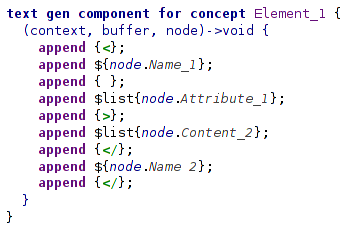
\includegraphics[width=90mm]{./img/textgen_example.png}
	\caption{Example of a~TextGen aspect}
	\label{fig:textgen_example}
\end{figure}

We can see that we gradually append all literals, properties, and children in the same order as they appear in the grammar definition.
This part of the process holds no first-hand complications.
We still need to generate BaseLanguage code dynamically, which in some cases might be a~challenge.
We figured how to overcome those challenges earlier in Section~\ref{chap:generating_code_inside_mps}.
There are, however, some hidden problems along the path.

\subsection{Whitespaces}
\label{chap:whitespaces}

As you might have noticed, there was no whitespace handling inside of our SimpleXML grammar.
For example in the \parserrule{element} rule, there is \lexerrule{Name} the element directly followed by \parserrule{attribute}*, but in the XML language we require at least one space as a~separator.
So how does the parser know how to split tokens, how many whitespace characters are expected, and which characters are whitespace in the first place?

\begin{itemize}
	\item How does our TextGen generator know that there should be a~space in between \parserrule{attribute} and \lexerrule{Name} but is not required between \literal{\textless} and \lexerrule{Name}?

	\item How does it know there is no space between quotes and an attribute value inside the \parserrule{attribute} rule?

	\item And how about multiple attributes --- do they need to be separated by spaces?
\end{itemize}

\subsubsection{Whitespace Handling in ANTLR}

We have left the whitespace handling part out earlier in order to keep things more simple as we were paying attention to the structure of the language in the first place.
There are two ways, how we can deal with whitespaces in ANTLR:

\begin{itemize}
	\item We can define special tokens that don't need to be used inside any parser rule.
	We mark them with special flag, telling the parser to skip these characters when this token is matched:

	\begin{antlr}
		\lexerrule{WHITESPACE}   :  \regex{[ {\textbackslash}r{\textbackslash}n{\textbackslash}t]+}   -> skip;
	\end{antlr}

	\item The second possibility is to create a~similar rule to the one above, but leaving out the skip flag.
	Then, we explicitly reference this token in every parser rule, where whitespace can occur.
	This sometimes means hundreds of different positions, so it is generally not a~recommended approach.
	There are however cases, where this is inevitable due to the nature of the ANTLR lexer.
\end{itemize}

\subsubsection{The Whitespace Problem}

The problem that arises here, is that the skip syntax hides the whitespace information from the grammar.
We have no way of tracing this information back.
If, on the other hand, we decided to go with the explicit definition, and put \lexerrule{WHITESPACE} tokens everywhere, we would encounter much bigger problem.
From the point of view of the TextGen aspect, it would help us a~bit, but not completely, as we still don't know what string represents the rule.
Secondly, when creating the structural aspect, we would create a~property for each of these token references as per Section~\ref{chap:common_ground}.
The effect of that would be that the imported MPS language will become unusable.
The code will be full of placeholders waiting for whitespace characters (even though they might be unnecessary, i.e. [0..n]).
\\

We could try harder and ask the user himself, whether there are any whitespace detecting rules or try detecting them ourselves.
But even this will not solve the problem, as the whitespace can be easily entangled inside non-whitespace tokens as shown below with the \parserrule{chardata} rule.
\\

If we look into existing ANTLR grammars, we can see that things get even more complicated.
ANTLR, just like as any other parser/lexer, gives us the possibility to switch the parsing context.
We are able to enter any user specified mode and then apply a~different set of rules depending on current mode, which gives us more flexibility.
This means we can handle whitespace both implicitly and explicitly at the same time inside one grammar based on the mode.
Secondly, there is the possibility of capturing whitespace together with other characters.
Consider the following excerpt from the official ANTLR XML grammar:

\begin{antlr}
	\parserrule{element}     :   \literal{<} \lexerrule{Name} \parserrule{attribute}* \literal{>} \parserrule{content}* \literal{</} \lexerrule{Name} \literal{>}
	            |   \literal{<} \lexerrule{Name} \parserrule{attribute}* \literal{/>}
	            ;

	\parserrule{content}     :   \parserrule{chardata}?
                ((\parserrule{element}? | \lexerrule{CDATA} | \lexerrule{COMMENT}) \parserrule{chardata}?)* ;

	\parserrule{chardata}    :   \lexerrule{TEXT} | \lexerrule{SEA{\_}WS} ;

	\lexerrule{TEXT}        :   \regex{~[<&]+} ;

	\lexerrule{SEA{\_}WS}      :   (\literal{ }|\literal{{\textbackslash}t}|\literal{{\textbackslash}r}? \literal{{\textbackslash}n})+ ;

	\lexerrule{OPEN}        :   \literal{<}             -> pushMode(INSIDE) ;

	mode INSIDE;
	\lexerrule{S}           :   \regex{[ {\textbackslash}t{\textbackslash}r{\textbackslash}n]}       -> skip ;
	\lexerrule{CLOSE}       :   \literal{<}             -> popMode ;
	\lexerrule{SLASH{\_}CLOSE} :   \literal{/>}            -> popMode ;
\end{antlr}

What is happening here, is that the author decided to skip whitespace characters only when we are inside of XML tags (see that the \parserrule{element} contains no explicit whitespace tokens).
On the outside, they are being cleverly swallowed by the \parserrule{chardata} rule (its second alternative) that wraps any content.
The \parserrule{content} rule is written a~bit differently from our SimpleXML version.
It is a~little bit more complicated, but the shorter structure, showing all the different ways we can express the grammar in.
\\

The problem we find here is that with all the features ANTLR has to offer, there are just too many ways, how we can handle whitespaces and they can get all mixed up together just like the previous example showed.
In the worst scenario, from the TextGen point of view, the language is skipping all whitespace characters silently and thus removing the information from the grammar completely.
\\

This leaves us with the original question and the root problem:
\\
\textbf{How does our TextGen aspect know between which children there must be a~whitespace and where it is forbidden so that the produced code is a~valid one?}

\subsubsection{Possible Improvements}

Following up on the question posed in the previous paragraph, we can ask ourselves a~different question.
If not our TextGen, how does the ANTLR parser know where whitespaces are due?
Surely the parser must know, otherwise, it wouldn't be able to tell wrong code from the right.
Well, the answer is that it knows once it starts parsing some code depending on the inner state of the parser.
Context modes make this quite simple.
They are quite easy to work with on runtime when we are actually parsing some source code, but it is impossible to determine the mode for rules statically.
In other words, it is impossible to detect, whether we are swallowing whitespaces silently for given rule or not.
This is caused by the possibility to jump between modes in almost any manner and therefore use one parser rule in different contexts.
\\

We do not, however, necessarily need to put different amounts of different whitespace characters in random places.
We only need to find places, where we are sure they must be at in order to make the code valid.
Then, we can put a~single space there.
Generally, it doesn't have to be a~space character, but since we are aiming for general purpose languages, we will go with the very frequently used space character.
We could get some hints from the way the lexer is splitting source code into tokens, which is happening practically statically too.
Consider the following setup:

\begin{antlr}
	\parserrule{element}    :   \literal{<} \lexerrule{Name} \parserrule{attribute}* \literal{>} \parserrule{content}* \literal{</} \lexerrule{Name} \literal{>} ;

	\parserrule{attribute}  :   \lexerrule{Name} \literal{="} \lexerrule{TEXT} \literal{"} ;

	\lexerrule{Name}       :   \regex{[:a-zA-Z]([:a-zA-Z]|-|{\_}|\textbackslash.|[0-9])*} ;

	\lexerrule{TEXT}       :   \regex{~[<"]*} ;
\end{antlr}

From the general knowledge of XML, we know that there is no space needed between the opening bracket of an XML tag and the name of the tag (i.e. \textbf{{\textless}img}).
On the other hand, there has to be one between the name of the tag and the name of the first attribute (i.e. \textbf{{\textless}img src=...}).
But why is that?
Simply, because the lexer needs to parse the input source into tokens using available lexer rules (regular expressions).
If it encounters a~whitespace, it will stop parsing previous token (unless there is space allowed in it), parse the whitespace one (throw it away when skipping) and continue with the next one.
\\

The reason the parser cannot differentiate tag name from attribute name without a~separator is caused by their regular expressions.
Consider a~string \textbf{A}, representing the tag name (a string that can be matched by the regular expression of the \lexerrule{Name} rule).
Let string \textbf{B} be a~string representing the attribute name.
Whenever \textbf{A} and \textbf{B} share some same characters, we cannot clearly state, where one ends and the other starts (when placed together).
More precisely, \textbf{A} can end with same characters as \textbf{B} can start with.
Even more precisely, some suffix of \textbf{A} can be some prefix of \textbf{B}.
In our case they are coincidently both given by the \lexerrule{Name} rule, but in general case we really care about any possible substrings.
\\

Determining whether a~suffix of a~string matched by one regular expression can be a~prefix of a~string matched by a~different regular expression is not an easy task.
We could try to generate strings that satisfy both regular expressions, but probably the only complete solution to this problem would be to construct automata representing both expressions.
Then we would need to examine them somehow, in order to detect similarity.
\\

Now what happens, if one of our children that can have zero cardinality, is empty (no element attributes)?
What are we going to do about whitespaces wrapping this child?
In this case we should probably do the same suffix/prefix comparison with the next-next child on the way, skipping the empty one.
Additionally let's not forget that all this logic needs to be contained in generated BaseLanguage code.
\\

We have decided to settle for a~more simple heuristics, which is described in Section~\ref{chap:textgen_solution}.

\subsection{Layout}

We have already established that whitespaces are hard to get right.
But how about the code layout itself?
What if we want to produce more readable code by adding i.e. indentation or line breaks?
Can we for example use the same information, we were mining when building the projectional editor?
It would seem like the editor and code layout are very close to each other and since we were unable to resolve editor problems fully (Section~\ref{chap:editor_aspect}), we won't be able to leverage the information here neither.

\subsubsection{Universal TextGen}
One idea, on how to approach layout inside the TextGen aspect, would be creating a~really smart universal TextGen method.
It would be static (always the same, independently of the grammar) and it would be the same for each concept of the language.
It could read the projectional editor definition and then somehow try to mimic this layout on output.
This might be quite straightforward, because each cell has its specific function that could be translated into a~text layout.
The added value of this approach would be that whenever user decides to adjust and improve the projectional editor, it would get automatically reflected inside this universal TextGen.
It would also have a~drawback that when user would want to change the TextGen definition for some concept, he would have to build it from scratch.
\\

After this proposal was discussed with JetBrains, it was immediately rejected.
The main reason for this being that aspects should be independent of each other.
This means that when someone would like to introduce an extension of a~language and change the editor, it might influence the TextGen in a~way that, it would start generating invalid code (e.g. we could for example easily remove the “if” keyword from the projectional part).
Sometimes we might also want to define more projectional editors and switch between them, which would also make this dysfunctional.
This is probably the reason that JetBrains haven't introduced their own universal TextGen so far (just like they introduced a~default projectional editor).

\subsection{Our Solution}
\label{chap:textgen_solution}

After the analysis, we have come to a~conclusion that the problem of TextGen layout is quite similar to the one we have seen with the projectional editor, described in Chapter~\ref{chap:editor_aspect}.
Since we are mostly dealing with text-based languages, their editor representation must be almost the same as their expected text output.
Once we would have some information about the layout for generating better projectional editor, we could leverage the same information and use it for TextGen improvement too.
We have, however, decided that adjusting the editor manually, after the import is done, is for now the fastest and the most efficient way how to deal with this problem, so we have no information to leverage here.
\\

Adjusting the layout, speaking in the terms of TextGen, means adding line breaks and indentation --- practically the same as what we are doing with the editor aspect.
Nonetheless, aside from layout, there is still the problem concerning whitespaces that we described above in Section~\ref{chap:whitespaces}.
We decided not to go into full depth and solve the problem using regular expression automata.
We have, however, tried to improve the situation using some really simple heuristics which gave surprisingly good results.
\\

We have started with a~very basic TextGen that would insert spaces in between every two elements of the concept.
Then we started restricting spaces on positions where we thought they are not needed.

\begin{enumerate}
	\item We have concluded that whenever there is a~literal, it is a~plain string token defined in the grammar that might, in most cases, get recognized by the parser safely without the need for a~whitespace separator around (think \textbf{'\textless'} in XML).
	So whenever there is a~non-alphabetical literal, we omit spaces around it.

	\item Next, we were looking at properties (non-literal, but regex lexer rules).
	These are strings inserted by the user of the language, whose form is constrained by a~regular expression (think XML tag's name).
	If these are neighboring a~literal rule, we look at that literal rule's content.
	We expect that the user will be inputting some alphabetical content (variable/method/class names, identificators, etc.).
	If the neighboring literal rule ends with an alphabetical character, we insert space, otherwise, we omit it.
	This will help in cases such as insides of quotes, next to semicolons or around brackets, but on the other hand, it will separate usual language keywords (function, var, in, etc.) from other content.

	\item We check for element emptiness (child not present) and do not insert spaces when elements are empty so that spaces do not accumulate.

	\item When two children concepts are next to each other, we always insert space.

	\item Sequences of children are separated with space.
	This is the place where we might later want to manually substitute it with a~line break.
	Think repeating \parserrule{content} inside an XML tag or list of XML attributes.
\end{enumerate}

These few simple heuristics have left us with some very nice results (tested mostly on XML, JSON, and JavaScript). Figure~\ref{fig:textgen_final} shows an example of a~TextGen aspect for the full SimpleXML element.
\\

\begin{figure}[ht]
	\centering
	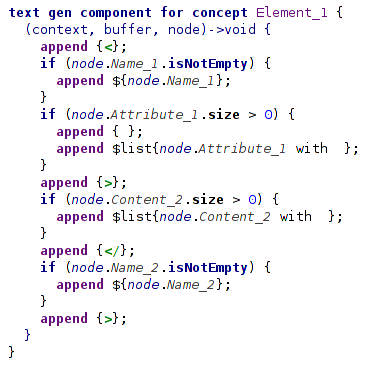
\includegraphics[width=95mm]{./img/textgen_final.png}
	\caption{Generated TextGen aspect for the SimpleXML element}
	\label{fig:textgen_final}
\end{figure}

If we wanted to manually adjust this generated code, so it generates nice indented XML code, we only need to wrap the \concept{Content{\_}2} child with indentation and change the sequence separator to a~new line character.
This is a~very fast and small adjustment, so we concluded that it is right to expect the user to do this kind of adjustments on his own.
Resulting adjusted aspect is shown below in Figure~\ref{fig:textgen_adjusted}.

\begin{figure}[t!]
	\centering
	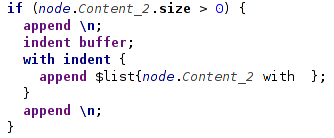
\includegraphics[width=85mm]{./img/textgen_adjusted.png}
	\caption{Adjusted indentation inside the TextGen aspect}
	\label{fig:textgen_adjusted}
\end{figure}
